\subsection{Waveforms Buck Converter, discontinuous inductor current}
In deze sectie analyseren we het gedrag van de buck converter onder licht gewijzigde omstandigheden ten opzichte van sectie 2.6. Hoewel de configuratie en het werkingsprincipe grotendeels hetzelfde blijven, zijn enkele parameters aangepast om de effecten hiervan op de inductorstroom \( I_L \) en andere belangrijke circuitwaarden te observeren. 

De gewijzigde componentwaarden worden weergegeven in Tabel \ref{tab:adjusted_component_values2}, en we voeren deze nieuwe waarden in de simulatie in om de bijbehorende golfvormen te genereren. Zoals in de vorige sectie (\autoref{2.6}) tonen we de relatie tussen \( I_L \) en belangrijke parameters zoals de uitgangsspanning \( V_{out} \), spanningspoot \( V_{leg} \), en de stromen door verschillende componenten binnen de converter.

\begin{table}[h!]
\centering
\begin{tabular}{|l|c|}
\hline
\textbf{Component} & \textbf{Value} \\ \hline
Vin & 48 V \\ \hline
L & 22 µH \\ \hline
C & 10 µF \\ \hline
Rout & 10 \(\Omega\) \\ \hline
Fs & 50 kHz \\ \hline
d & 40\% \\ \hline
\end{tabular}
\caption{Component values for the circuit}
\label{tab:adjusted_component_values2}
\end{table}

\begin{figure}[h!]
    \centering
    \begin{subfigure}[b]{0.45\linewidth}
        \centering
        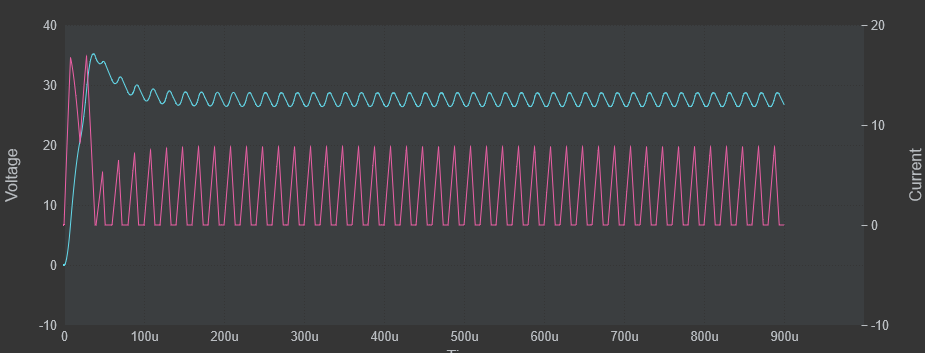
\includegraphics[width=\linewidth]{img/hfd2/IL-VOUT-7.png}
        \caption{Waveform of \(I_{L}\) and \(V_{\text{OUT}}\)}
        \label{fig:Waveform_IL_VOUT}
    \end{subfigure}%
    \hfill
    \begin{subfigure}[b]{0.45\linewidth}
        \centering
        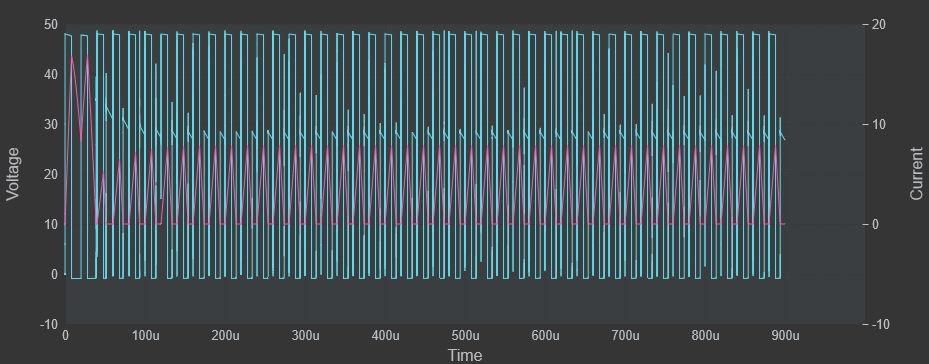
\includegraphics[width=\linewidth]{img/hfd2/IL-VLeg-7.png}
        \caption{Waveform of \(I_{L}\) and \(V_{\text{Leg}}\)}
        \label{fig:Waveform_IL_VLeg2}
    \end{subfigure}
    
    \caption{Waveforms comparing \(I_{L}\) with \(V_{\text{OUT}}\) and \(V_{\text{Leg}}\)}
    \label{fig:Waveforms_IL_VOUT_VLeg}
\end{figure}

\begin{figure}[h!]
    \centering
    \begin{subfigure}{0.45\linewidth}
        \centering
        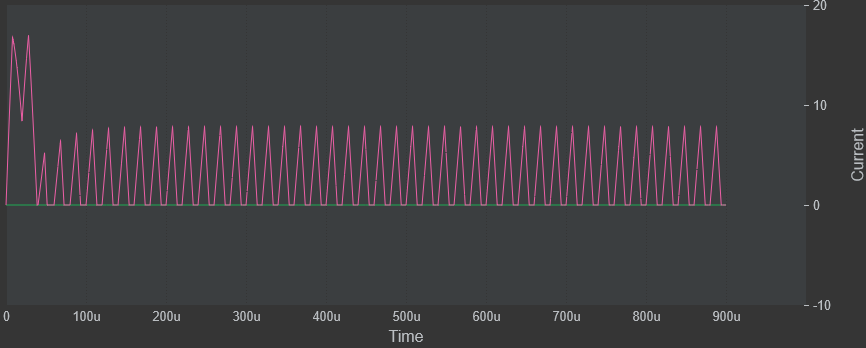
\includegraphics[width=\linewidth]{img/hfd2/IL-IDS-7.png}
        \caption{Current through MOSFET (IL-IDS) during simulation}
        \label{fig:IL-IDS-7}
    \end{subfigure}
    \begin{subfigure}{0.45\linewidth}
        \centering
        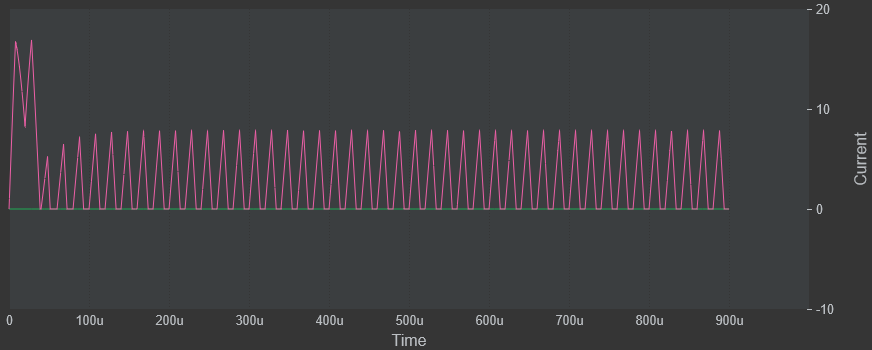
\includegraphics[width=\linewidth]{img/hfd2/IL-ID-7.png}
        \caption{Current through Diode (IL-ID) during simulation}
        \label{fig:IL-ID-7}
    \end{subfigure}
    \begin{subfigure}{0.45\linewidth}
        \centering
        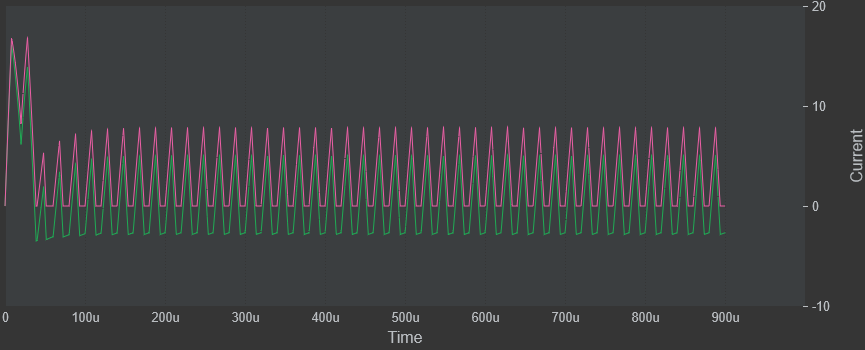
\includegraphics[width=\linewidth]{img/hfd2/IL-IC-7.png}
        \caption{Current through Output Capacitor (IL-IC) during simulation}
        \label{fig:IL-IC-7}
    \end{subfigure}
    \begin{subfigure}{0.45\linewidth}
        \centering
        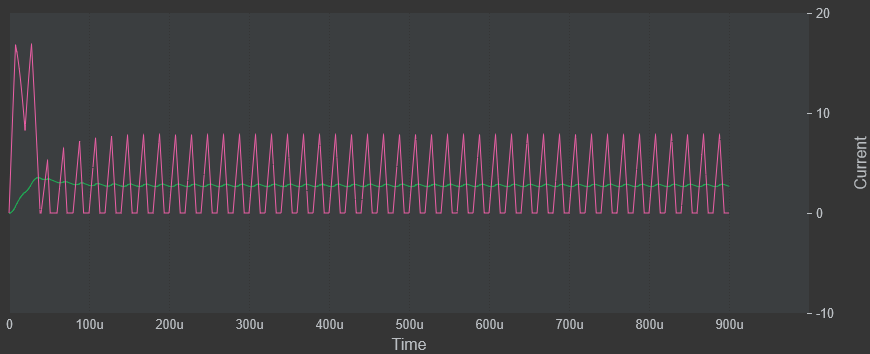
\includegraphics[width=\linewidth]{img/hfd2/IL-IR-7.png}
        \caption{Current through Output Resistor (IL-IR) during simulation}
        \label{fig:IL-IR-7}
    \end{subfigure}
    \begin{subfigure}{0.45\linewidth}
        \centering
        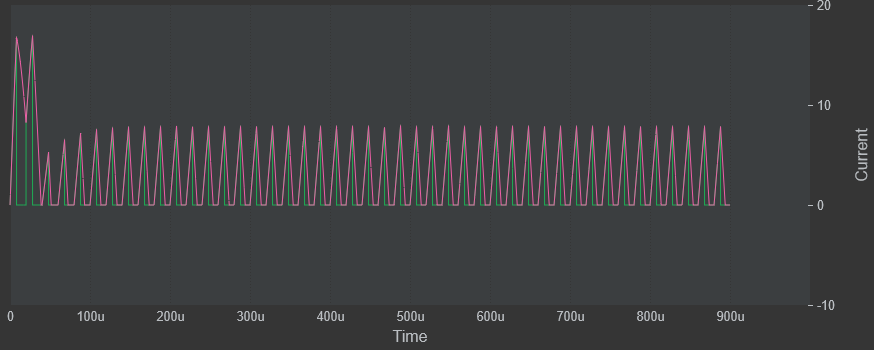
\includegraphics[width=\linewidth]{img/hfd2/IL-Lin-7.png}
        \caption{Current through Input Voltage Source (IL-Iin) during simulation}
        \label{fig:IL-Lin-7}
    \end{subfigure}
    
    \caption{Current measurement waveforms for various components in the simulation setup}
    \label{fig:adjusted_waveforms2}
\end{figure}
De golfvormen verkregen uit deze simulatie worden gepresenteerd in Figuur \ref{fig:adjusted_waveforms2}. Deze vergelijkingen laten zien hoe de aangepaste parameters het stroomverloop in het circuit beïnvloeden, en bieden verdere inzichten in de stabiliteit en efficiëntie van de converter onder deze nieuwe omstandigheden.